\documentclass[tikz,border=10pt]{standalone}
\usepackage{tikz}
\usetikzlibrary{shapes,arrows,positioning,decorations.pathreplacing}
\usepackage{amsmath}

\definecolor{fepblue}{RGB}{41,128,185}
\definecolor{crrgreen}{RGB}{39,174,96}
\definecolor{goalred}{RGB}{192,57,43}
\definecolor{matchpurple}{RGB}{142,68,173}

\begin{document}
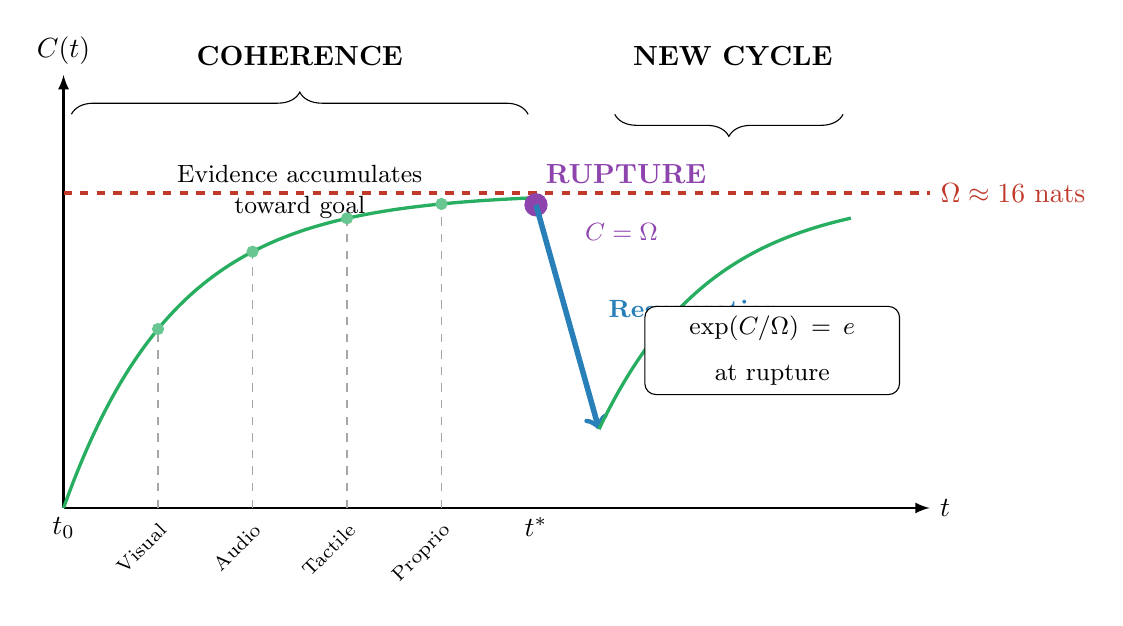
\begin{tikzpicture}[scale=1]
% Time axis
\draw[-latex, thick] (0,0) -- (11,0) node[right] {$t$};
\draw[-latex, thick] (0,0) -- (0,5.5) node[above] {$C(t)$};

% Omega threshold
\draw[dashed, very thick, goalred] (0,4) -- (11,4) node[right] {$\Omega \approx 16$ nats};

% Coherence curve
\draw[very thick, crrgreen, domain=0:6, samples=100]
    plot (\x, {4*(1 - exp(-0.7*\x))});

% Rupture point
\filldraw[matchpurple] (6,3.85) circle (4pt);
\node[above right, matchpurple, font=\bfseries] at (6,4) {RUPTURE};
\node[right, matchpurple, font=\small] at (6.5,3.5) {$C = \Omega$};

% Regeneration arrow
\draw[very thick, fepblue, ->, line width=2pt] (6,3.85) -- (6.8,1);
\node[fepblue, font=\small\bfseries, right] at (6.8,2.5) {Regeneration};

% New cycle
\draw[very thick, crrgreen, domain=6.8:10, samples=100]
    plot (\x, {1 + 3*(1 - exp(-0.7*(\x-6.8)))});

% Labels
\node[below] at (0,0) {$t_0$};
\node[below] at (6,0) {$t^*$};

% Phase labels
\draw[decorate, decoration={brace, amplitude=8pt}] (0.1,5) -- (5.9,5);
\node[above, font=\bfseries] at (3,5.5) {COHERENCE};
\node[below=15pt, font=\small, text width=35mm, align=center] at (3,5) {Evidence accumulates\\toward goal};

\draw[decorate, decoration={brace, amplitude=8pt, mirror}] (7,5) -- (9.9,5);
\node[above, font=\bfseries] at (8.5,5.5) {NEW CYCLE};

% Evidence markers with labels
\foreach \x/\label in {1.2/Visual, 2.4/Audio, 3.6/Tactile, 4.8/Proprio} {
    \draw[gray!70, dashed] (\x,0) -- (\x,{4*(1 - exp(-0.7*\x))});
    \node[below, font=\scriptsize, rotate=45, anchor=north east] at (\x,0) {\label};
    \filldraw[crrgreen!70] (\x,{4*(1 - exp(-0.7*\x))}) circle (2pt);
}

% Annotation box
\node[draw, rounded corners, fill=white, font=\small, text width=30mm, align=center] at (9,2) {
$\exp(C/\Omega) = e$\\[2mm]
at rupture
};
\end{tikzpicture}
\end{document}
